\documentclass[a4paper,12pt]{article}

% Packages
\usepackage{float}  % For precise figure placement
\usepackage[T1]{fontenc}
\usepackage{lmodern}
\usepackage[utf8]{inputenc}
\usepackage{graphicx}  % For images
\usepackage{listings}  % For code snippets
\usepackage{xcolor}    % For code coloring
\usepackage{hyperref}  % For hyperlinks
\usepackage{amsmath}   % For math equations
\usepackage{caption}   % Better captions
\usepackage{geometry}  % Page layout
\geometry{margin=2.5cm}

% Remove paragraph indentation
\setlength{\parindent}{0pt}

% Code styling
\lstset{
    language=Python,
    basicstyle=\ttfamily\footnotesize,
    keywordstyle=\color{blue},
    stringstyle=\color{red},
    commentstyle=\color{gray},
    breaklines=true,
    frame=single
}

\title{Lab Report: \textbf{Weather Station – Lab 1}}
\author{Gautam Shailendra Sharma \\ Matriculation No.: 12505118 \\ Course Name \\ Instructor: Prof. Tobias Schaffer}
\date{08 June 2025}

\begin{document}

\maketitle
\vspace{1cm} 
\section{Introduction}
In this lab, we utilized the Raspberry Pi with the Sense HAT to collect environmental sensor data such as humidity, temperature, and pressure. The data was then displayed in real time on the LED matrix of the Sense HAT.

\section{Methodology}

\subsection{Software and Hardware Used}
\begin{itemize}
    \item Programming language: Python, SSH Command Line
    \item Libraries: SenseHat, time, matplotlib
    \item Hardware: Raspberry Pi 5, Sense HAT
\end{itemize}

\subsection{Code Repository}
The full source code for this project is available on GitHub at:

\begin{center}
\href{https://github.com/GRODER/thd-em-lab1-weather-station}{\texttt{https://github.com/GRODER/thd-em-lab1-weather-station}}
\end{center}

This repository includes:
\begin{itemize}
    \item Source code files
    \item Documentation and usage guidelines
    \vspace{10cm} 
\end{itemize}

\subsection{Code Implementation}

\begin{lstlisting}[language=Python]
from sense_hat import SenseHat
import time
import matplotlib.pyplot as plt

sense = SenseHat()

temperature_readings = []
humidity_readings = []
pressure_readings = []
time_reading = []

actual_temp = 13.1
actual_humidity = 65
actual_pressure = 1016

for i in range(1, 11):
    print(f"iteration {i}")
    temp = sense.get_temperature()
    humidity = sense.get_humidity()
    pressure = sense.get_pressure()
    
    sense.show_message(f"Temp : {temp: .1f}C", scroll_speed=0.08, text_colour=(255,160,122))
    temperature_readings.append(temp)
    
    sense.show_message(f"Hum. : {humidity: .1f}%", scroll_speed=0.08, text_colour=(64,224,208))
    humidity_readings.append(humidity)
    
    sense.show_message(f"Press. : {pressure: .1f}HPa", scroll_speed=0.08, text_colour=(182,12,47))
    pressure_readings.append(pressure)
    
    time_reading.append(i)
    time.sleep(1)

# Calculate averages
avg_temp = sum(temperature_readings) / len(temperature_readings)
avg_humidity = sum(humidity_readings) / len(humidity_readings)
avg_pressure = sum(pressure_readings) / len(pressure_readings)

print(f"\nCalculated Temp: {avg_temp:.1f}C \t Actual Temp: {actual_temp:.1f}C")
print(f"Calculated Humidity: {avg_humidity:.1f}% \t Actual Humidity: {actual_humidity:.1f}%")
print(f"Calculated Pressure: {avg_pressure:.1f}hPa \t Actual Pressure {actual_pressure:.1f}hPa")

# Plotting
plt.figure(figsize=(15,10))

# Temperature plot
plt.subplot(3,1,1)
plt.plot(time_reading, temperature_readings, marker='o', label="Measured Temperature", color="blue")
plt.axhline(y=actual_temp, color="red", linestyle='--', label="Actual Temperature")
plt.title("Temperature Readings over Time")
plt.xlabel("Time (sec)")
plt.ylabel("Temperature (°C)")
plt.legend()
plt.grid()

# Humidity plot
plt.subplot(3,1,2)
plt.plot(time_reading, humidity_readings, marker='o', label="Measured Humidity", color="blue")
plt.axhline(y=actual_humidity, color="red", linestyle='--', label="Actual Humidity")
plt.title("Humidity Readings over Time")
plt.xlabel("Time (sec)")
plt.ylabel("Humidity (%)")
plt.legend()
plt.grid()

# Pressure plot
plt.subplot(3,1,3)
plt.plot(time_reading, pressure_readings, marker='o', label="Measured Pressure", color="blue")
plt.axhline(y=actual_pressure, color="red", linestyle='--', label="Actual Pressure")
plt.title("Pressure Readings over Time")
plt.xlabel("Time (sec)")
plt.ylabel("Pressure (hPa)")
plt.legend()
plt.grid()

plt.tight_layout()
plt.show()
\end{lstlisting}

\section{Results}

Figure \ref{fig:terminal} shows the raw sensor values being printed on the Raspberry Pi terminal during the 10-second sampling period. These include the measured values of temperature, humidity, and pressure.

Figure \ref{fig:graph} presents the plotted graph comparing the measured values from the Sense HAT sensors with the actual reference values. Each subplot corresponds to a specific parameter (temperature, humidity, and pressure), along with horizontal dashed lines representing the actual values for visual comparison.

\begin{figure}[H]
    \centering
    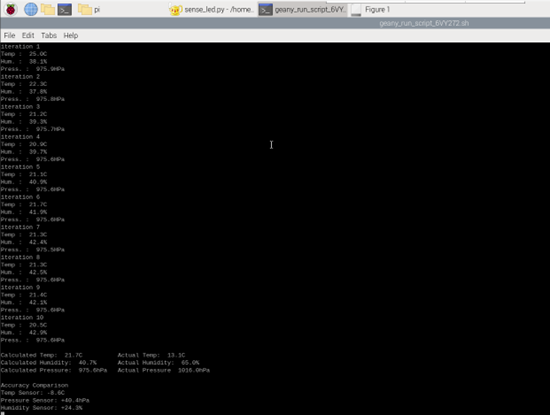
\includegraphics[width=\textwidth]{images/terminal_readings.png}
    \caption{Sensor readings printed on the Raspberry Pi terminal}
    \label{fig:terminal}
\end{figure}

\vspace{0.8cm}

\begin{figure}[H]
    \centering
    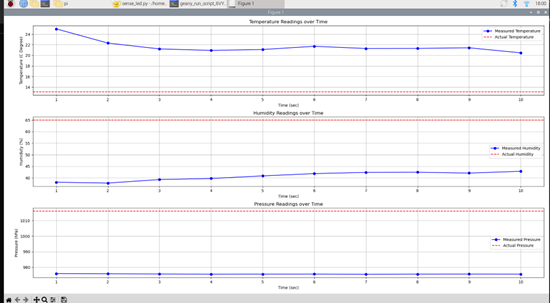
\includegraphics[width=\textwidth]{images/sensor_graph.png}
    \caption{Measured vs Actual values of Temperature, Pressure and Humidity}
    \label{fig:graph}
\end{figure}

\section{Challenges, Limitations, and Error Analysis}



\subsection{Challenges Faced}
\begin{itemize}
    \item IP address discovery failed when trying to connect the Raspberry Pi via SSH.
    \item Resolution: Used hostname in PuTTY to retrieve the assigned IP address.
\end{itemize}

\subsection{Error Analysis}
\begin{itemize}
    \item Mistyped syntax in function calls like \texttt{print()} and \texttt{sense.show\_message()} caused temporary runtime errors during development.
    
    \item A significant discrepancy was observed between the actual temperature and the value reported by the Sense HAT. This is due to the sensor being located close to the Raspberry Pi's components, causing it to initially pick up heat from the board rather than ambient temperature.

    \item Upon blowing air over the board, the temperature readings dropped noticeably (by around 2.8°C) as the heat was dissipated from the sensor's surroundings. This indicates that heat accumulation around the Sense HAT can severely affect its readings.

    \item If proper ventilation or cooling is provided, the sensor readings may converge towards the actual values with time. This suggests that additional sampling iterations — along with an effective heat dissipation strategy — could lead to more accurate temperature measurements.
\end{itemize}

\section{Discussion}

The Sense HAT sensor readings displayed the following properties:

\begin{itemize}
    \item \textbf{Repeatability:} Sensor readings remained consistent across multiple iterations, indicating stable internal sensing behavior.

    \item \textbf{Accuracy:} The manufacturer-specified accuracies are:
    \begin{itemize}
        \item Temperature: ±0.5°C
        \item Pressure: ±1 hPa
        \item Humidity: ±3\% RH
    \end{itemize}

    \item \textbf{Observed Deviations:} There was a noticeable difference between actual and measured values, especially for temperature. For example:
    \begin{itemize}
        \item Temperature: +24.4°C error
        \item Pressure: –41.4 hPa error
        \item Humidity: –35.3\% error
    \end{itemize}

    \item \textbf{Thermal Influence:} Initially, the temperature readings were significantly higher due to the influence of the Raspberry Pi’s components heating the sensor. However, when air was blown over the board, the readings began to drop, suggesting a dissipation of localized heat.

    \item \textbf{Convergence Behavior:} With more sampling iterations, and provided that heat is efficiently dissipated from the board (via ventilation or passive cooling), the Sense HAT temperature readings appear to converge toward actual environmental values. This makes it useful for long-term monitoring in thermally stable environments.
\end{itemize}

\section{Conclusion}
This lab provided practical exposure to real-time data collection and sensor behavior analysis using the Raspberry Pi and Sense HAT. Despite known hardware limitations, useful patterns and discrepancies were identified, forming the basis for calibration strategies in future setups.

\section{References}
\begin{itemize}
    \item Raspberry Pi Foundation. \url{https://www.raspberrypi.com}
    \item Sense HAT Documentation. \url{https://pythonhosted.org/sense-hat/}
    \item Datasheet of ST Temp \& Humidity sensor (HTS221) and Pressure sensor(LPS25H) 
\end{itemize}

\end{document}